\subsection{Program Design}
%%NEILL: paragraph or two about overall system architecture, e.g. what runs on-board the drone, what's off-board, what's being done runtime, what's been pre-processed (e.g. clustering is trained beforehand)

The dancing drone software solution is broken down into three main modules; the audio module, drone dancer
module and classification module. These modules are all used by a single main script/routine which specifies
what audio to dance to, and the 'mood' of the dancing. All software discussed in this guide ran on a laptop
separate to the drone. While code is able to be compiled to run natively on the ARDrone's ARM processor, the
sensor protocols and actuator control are not documented by Parrot and much of the software running on the
ARDrone is closed source. As Parrot supports controlling the drone over its WiFi network, it was decided that the
code will all be run on a separate device to the drone. Each module discussed below runs asyhcnronously to
prevent from `sleep' functions in the code stalling the music playback or adding a delay before the drone does a
move. By running each module in a different thread, synchronization between music playback and drone movements
can be achieved through event-driven programming rather than looking ahead in the audio file and trying to
predict the next position of the drone in order to make it move in time.\\

\subsubsection{Audio Module}
The audio module performs pre-processing on a given audio file, or live processing on an audio stream from a
microphone or line in. The audio module uses the Aubio library, a free open-source audio processor. The Aubio
module is further discussed in the 'Tempo Detection' section later in this report. The audio module works
together with the classification module to determine whether the current point in the song is a chorus or a
sparse section. At any point during playback, the current time, bpm and section label (chorus or sparse) can be
retrieved. In the case of live audio processing, the current time is not relevant as beat/onset events are fired
when detected. \\

For live processing, the audio module delays outgoing audio (in the case of using line-in). In the case of
reading audio from a microphone, no lookahead can be implemented as the audio cannot be delayed as it is coming
from an external, audile source. Line-in audio is able to be delayed as it is played by the audio module, and is
not audible unless the line-in is configured to be so in the sound settings of the computer being used. Lookahead
was needed for accurate bpm representation of live audio where the bpm varies over the song or between sections.
The reasons for this are outlined in the 'Tempo Detection' section further in this report, where the limitations
of the Aubio library are discussed. The code behind the audio module is viewable at \eqref{code:play_song.py}\\

The audio module also handles synchronization of events that should be performed to the beat, or on the onset of
a beat. Function pointers can be given to the audio module to be executed when it detects a beat or onset of a
beat (depending on if the current bpm is regular enough to use). An example of the audio beat event function hook
is shown below, with input generated by clapping next to the microphone.\\

\begin{figure}[h]
    \centering
    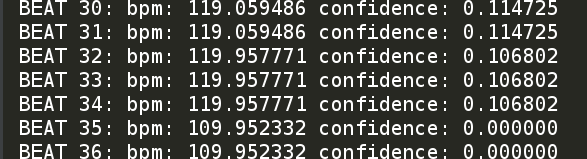
\includegraphics[scale=0.3]{BEAT}
    \caption{The audio beat event firing, triggered by clapping near the microphone. Notice that when the bpm
    changes significantly, the bpm confidence drops to 0.}
\end{figure}

\subsubsection{Drone Dancer Module}
The drone dancer module is responsible for all physical movements of the drone. One of the main limitations of
the ARDrone.2 encountered was the internal command-queue behaving inconsistently. According to Parrot's
documentation, when using the in-built animations of the drone (backflip, bob nose down etc.), the animation code
and duration must be specified in order to let the drone know how long to wait until attempting to perform the
next animation. The drone did not always behave consistently and wait for the specified duration between moves,
and sometimes required strange values to work. An example of this is performing flips, a duration of 15ms must be
given (as opposed to 1000ms or 6s as specified in Parrot's SDK examples) and then a 'hover' command sent 0.45s
later. Operations such as this are abstracted by the drone dancer module, which implements a queue of moves to
do, sleeping for the appropriate amount of time when each one is sent. At any time dancing can be paused and
resumed without affecting the moves in the queue.\\

The move queue is one of the main motivators for making the dancing drone solution multi-threaded. As the drone
dancer module runs in its own thread, any sleeps performed within it do not affect the audio playback or
operation of the rest of the program.\\

The drone dancer contains definitions for each kind of move the drone can do, and some functions that when called
repeatedly dance in a certain 'mood'. Each move takes varying arguments, for example wiggling to a certain
frequency, or bobbing in a different direction each time the same function is called. These parameters can be
given manually or can be generated automatically by the drone dancer class using the current bpm or onset given by the
audio module. The drone's dancing is generally driven by a function being called on the beat or on the onset of a
beat by the audio module, as discussed in the previous section. For the code behind the drone dancer module, see
\eqref{code:drone_dancer.py}.\\

The drone dancer class is also responsible for navigation of the drone. Using a separate thread, the navigation
data is constantly read in from the drone. If a roundel is detected on the ground, the dancing thread is blocked
until the navigation thread has moved the drone back into a safe location.\\

\subsubsection{Classification Module}
The classification module performs cluster analysis on the last 10 chunks in the current audio stream to
determine whether they are likely to be a chorus or sparse section. The classification module had to be trained before
use, but is able to classify song sections in real time. The operation of the classification module is further
discussed in the sound processing section further in this report. The code behind the cluster module is viewable
at \eqref{code:cluster.py}.\\

\subsubsection{Routine}
The main routine file is what uses all the modules together from their public interfaces in order to make the
drone dance in a certain situation. An example routine file is viewable at \eqref{code:routine_hardstyle.py}.

A data flow diagram showing the high-level communication between each module is shown overleaf.

\onecolumn
\begin{figure*}[h]
\begin{tikzpicture}

\draw  (-1.5,6.5) circle [radius=1.5] node {Routine / Main};
\draw  (-1.5,2.5) circle [radius=1.5] node {Audio};
\draw  (-7,2.5) circle [radius=1.5] node {Classification};
\draw  (3.5,2.5) circle [radius=1.5] node {Drone Dancer};



\node at (-5.5,5.5) {Audio File};
\draw [->] (-3.0,6.5) -- (-6.0,3.7);


\node at (-3.7,4.5) {Audio File};
\draw [->] (-2.7,5.6) -- (-2.7,3.5);


\node at (-4.2,3) {Song Structure};
\draw [->] (-5.5,2.5) -- (-3,2.5);

\node at (1,3) {\begin{tabular}{c}Beat/Onset\\Events\end{tabular}};
\draw [->] (0,2.5) -- (2,2.5);


\node at (1.5,6) {Dance Style};
\draw [->] (-0.1,6) -- (2.6,3.8);


\node at (6.2,0.5) {Movement Commands};
\draw [->] (3.5,1) -- (3.5,-0.5);

\draw  (2,-0.5) rectangle (5,-2) node[pos=.5] {Drone};
\end{tikzpicture}
\caption{High level Data Flow Diagram of the dancing drone solution.}
\end{figure*}

\begin{multicols}{2}
\twocolumn

\end{multicols}
\clearpage
